\documentclass[12pt]{article}

\usepackage[a4paper, left=2.5cm, right=2.5cm, top=2.5cm, bottom=2cm]{geometry}
\usepackage{graphicx}
\graphicspath{ {./} }

\begin{document}

\begin{titlepage}
\centering
\vspace*{6cm}
{\huge\bfseries BACnet Blocklists\par}

\vspace{3cm}

{\Large Introduction to Internet and Security}\\
\vspace{0.1cm}
{\Large Prof. Dr. Christian Tschudin}\\
\vspace{0.2cm}
{\Large FS 2021}\\
\vspace{0.1cm}
{\Large University of Basel}

\vspace{1cm}

{\large Group 12: Jannick Heisch, Paul Tr\"oger}

\vspace{1cm}

{\large 18.07.2021}

\end{titlepage}


\section{Introduction}
At the beginning, the Internet was characterized by a decentralized structure but became more and more centralized over time.
This causes a problem when governments censor the Internet and restrict access to certain content, particularly the communication in social networks. 
The goal of BACnet is to create a decentralized network, based on the Secure Scuttlebutt protocol, to circumvent control by few organizations or governments and to ensure communication independent of the Internet. \\
The BACnet project is the result of several subprojects in which different groups of students work together. 
Because of the increasing amount of harassment and discrimination in today’s Internet, especially in social media, our group aims to improve this project by implementing blocklists. 
The goal of blocklists is to block inappropriate content (harassment, discrimination, racism, insults) and prevent it from spreading across the network.

\section{Background}
The BACnet network structure consists of sequences of events that are chained together to feeds. 
Each feed has an ID, which uniquely identifies the user of the feed. 
This identification process allows us to block users and their content --- whenever it is necessary. \\
\\
Content of the Internet can be easily changed or removed such as methods used by Facebook, Twitter, etc. 
On the contrary, the feeds of the BACnet network structure are append-only logs.
This poses a substantial challenge for the blocklist implementation since messages cannot be edited or removed from the log without violating data integrity. 
Therefore, we needed an alternative method in order to preserve data integrity.\\
\\
Since JSON is easy to use in python, we decided to additionally implement the import and export of blocked words and authors using JSON files. 
This allows you to share and extend your own blocklist from other sources beyond BACnet, such as external word lists which already contain a large number of inappropriate expressions.

\section{Implementation}
Our finished module is meant to be used as a library. It is divided into two parts: \\
1. The blocklist, which is used to store words and users that should be blocked. \\
2. The block settings, which determine how the content is filtered and distributed. \\
The functions in our module can be used to edit and save blocklists and block settings, as well as to filter events, feeds and content. It is also possible to share and import blocklists with the help of our module.

\subsection{Documentation}
Since this is a group project, documentation is essential for the group itself, but also for the people who will continue working with this module. 
Therefore, all methods are commented using Python comments and we created a document describing how the blocklist module is used.

\subsection{Blocklist}
The blocklist class is responsible for creating and editing blocklists as well as filtering content. 
These lists, which contain blocked words and IDs of authors, can be loaded from and saved as JSON files or BACnet feeds. In addition, blocklists from other sources can be imported and combined with your own list. 
This allows the sharing of lists with other people. \\
\\
The filter methods filter messages that contain blocked words or are written by blocked authors. The filtered content can only be used for the display of the content. It is not possible to overwrite the original feed with the filtered version, because the data integrity of the Scuttlebutt protocol would be violated. Every user receives the original message, which is displayed after it went through the user’s blocklist. \\
Because deleting events is not possible we have introduced the concept of \textit{suggestion block}. This allows to transfer the information to other users that certain messages may contain inappropriate content without changing the original feed.\\ Thus, the protocol is not violated. \\
For example: Bob is receiving and filtering the log of Alice. With the help of his blocklist, he saves the sequence numbers of her events, which contain blocked words, into a new event in his feed. 
Now, John filters the feed of Alice. Depending on how he has set his block settings, the suggestions of Bob are considered in addition to his own block list.

\subsection{Blocksettings}
The block settings allow the user to customize the filtering of the content.\\
The settings consist of two parts: The block settings and the suggestion block settings. \\
The block settings enable the user to choose how the content is filtered with their block list.\\ There are three setting options: \\
1. Noblock: Filtering with the help of the own blocklist is disabled. \\
2. Softblock: Words, which are part of the blocklist, are censored without deleting the whole message. If the author is part of the blocklist, the whole message will be deleted.\\
3. Hardblock: If words or authors are part of the blocklist, the whole message will be deleted.\\
\\
With the help of the suggestion block settings, the user can determine whether he wants to take over suggestions from other users or not. The settings are saved in the own feed and remain persistent.


\section{Result}

\subsection{Blocklist sharing}
\vspace{0.5cm}
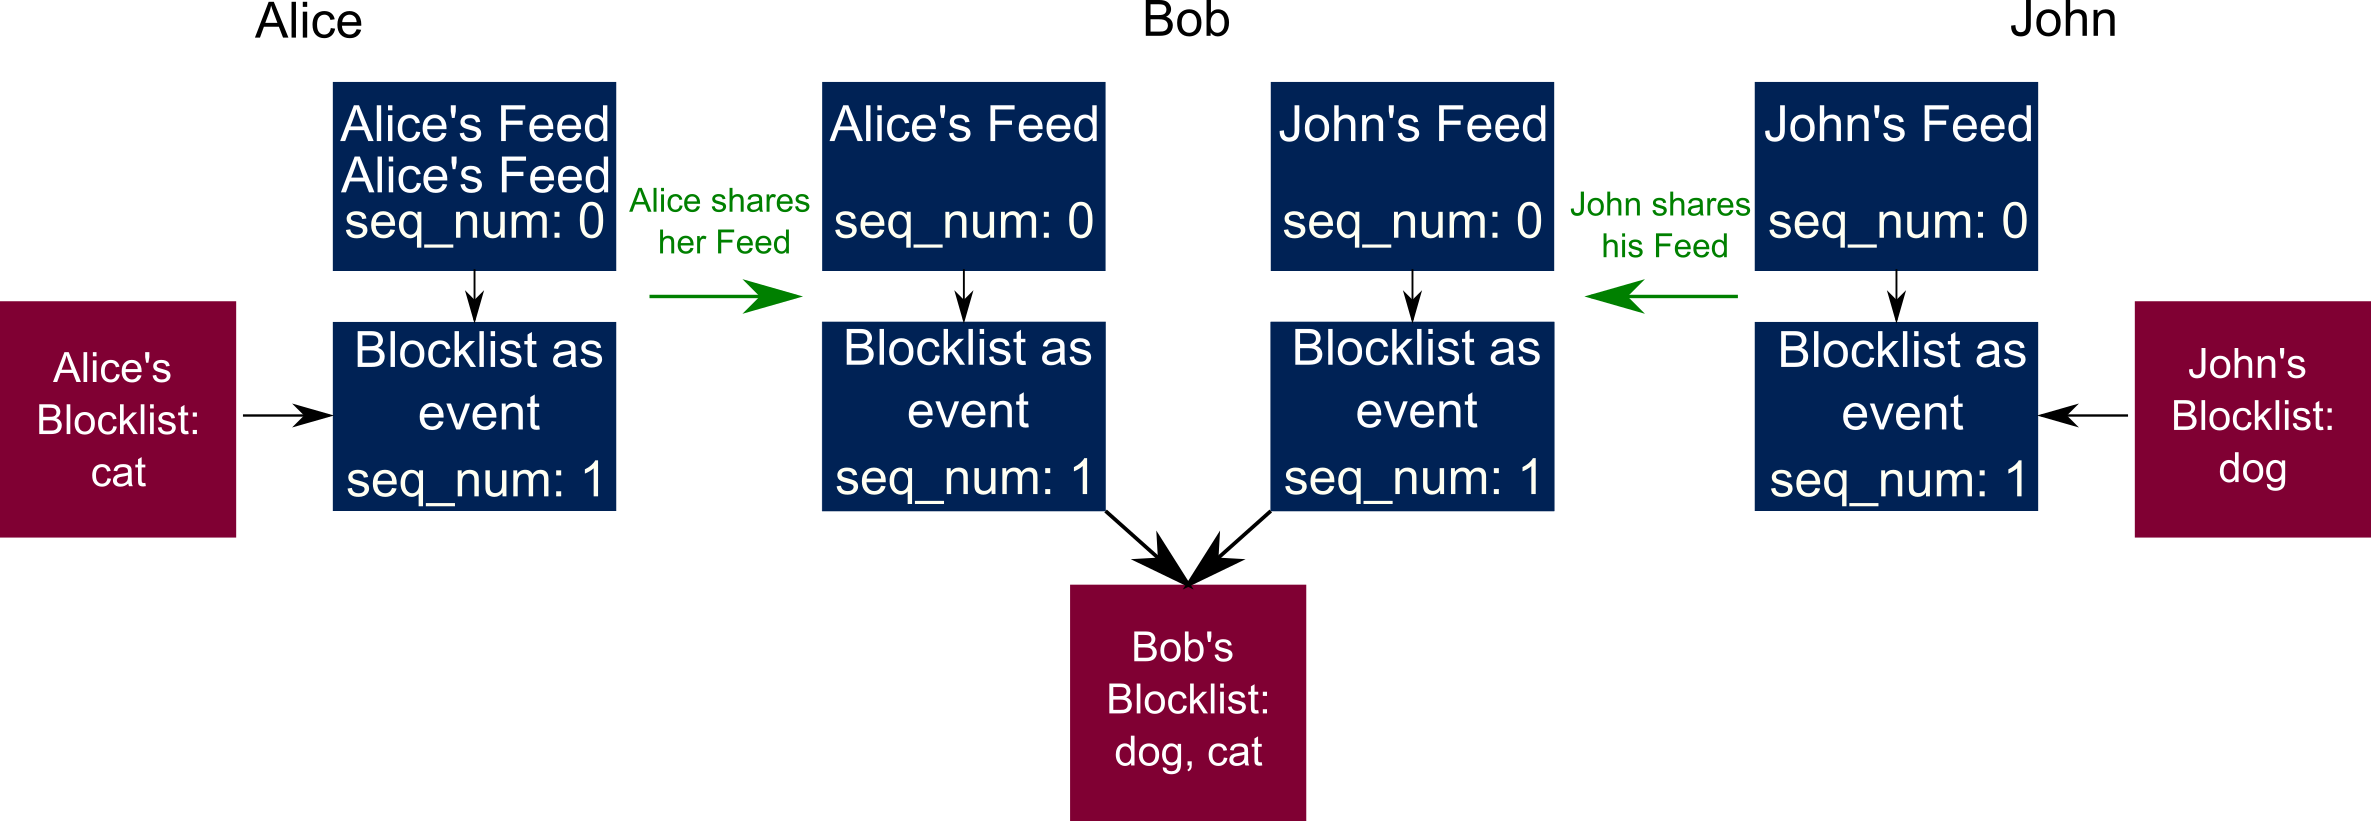
\includegraphics[width=\textwidth]{graph2}\vspace{0.5cm}
This example shows how Blocklists can be shared over the secure scuttlebutt protocol.
The initial situation is that Bob does not yet have a block list. Alice and John, however, have two distinct ones.
Both Alice and John write their Blocklists into their feed.
After sharing them with Bob, he merges both Lists to use as his own.


\subsection{Suggested Blocking}
\vspace{0.5cm}
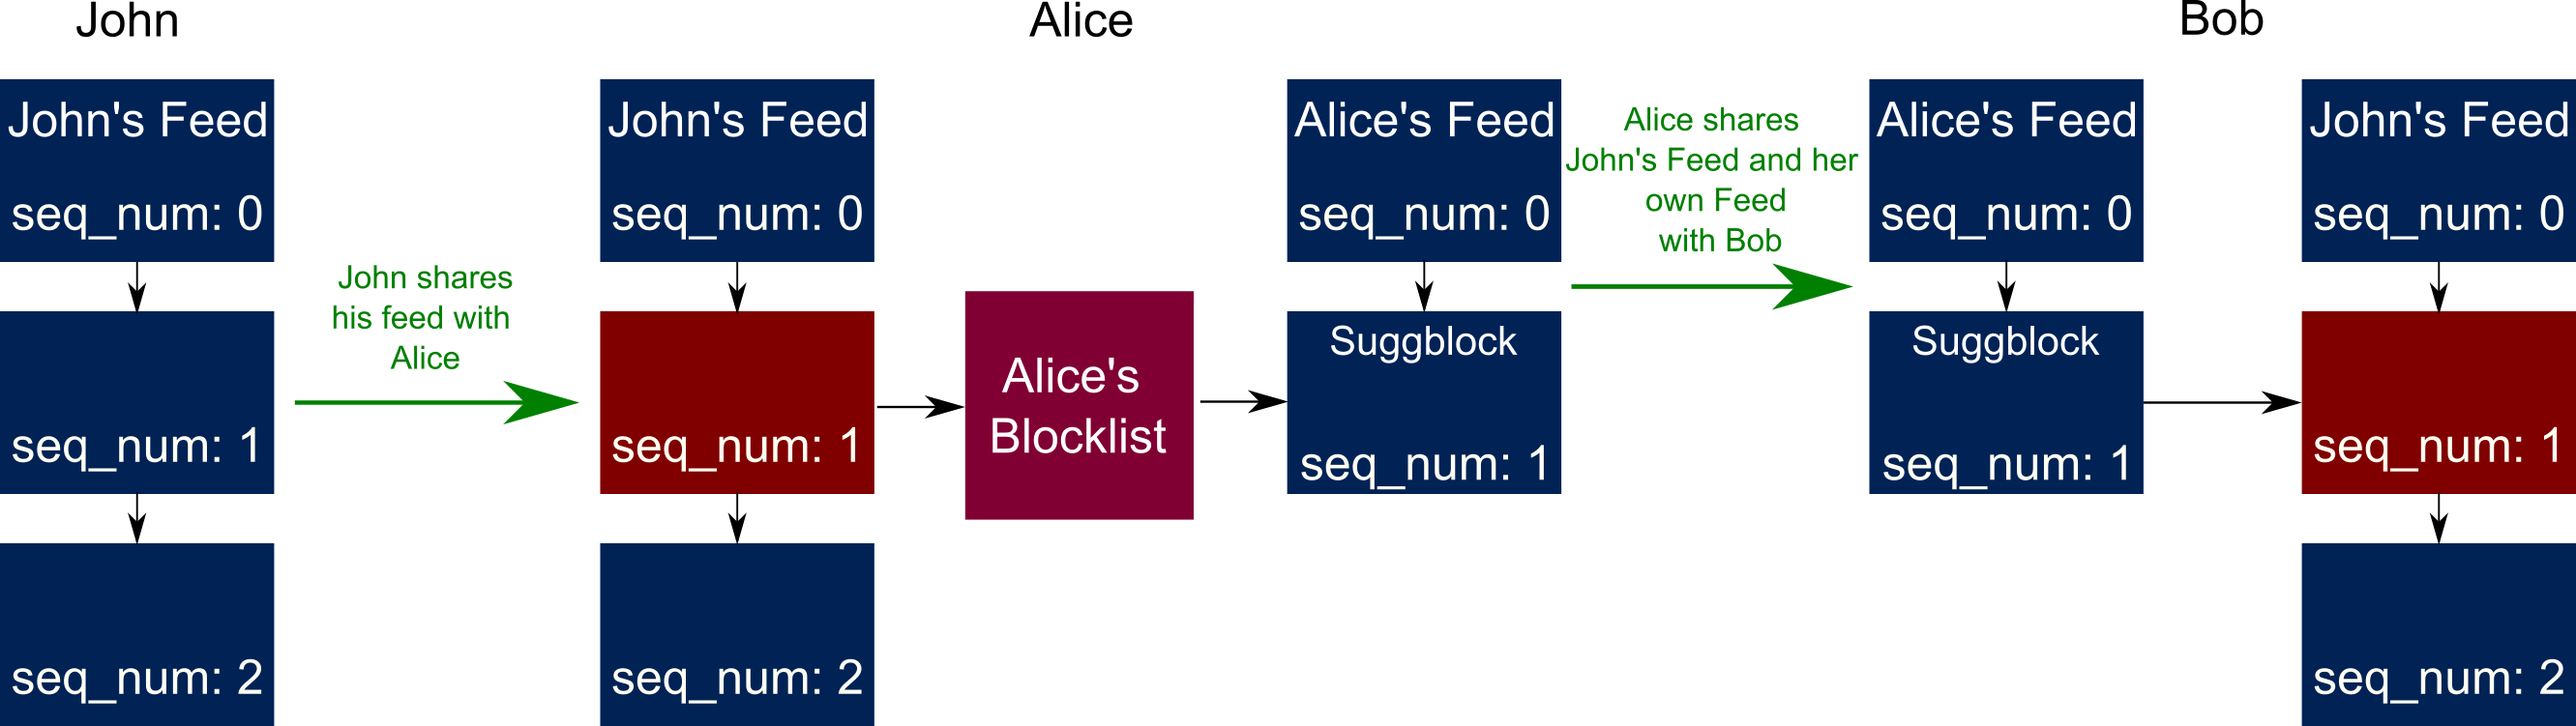
\includegraphics[width=\textwidth]{graph1}\vspace{0.5cm}
Here you can see how someone can block entries from being shared by using the suggestion block feature.
John sends his feed to Alice. Alice uses her own blocklist to determine that entry 1 should be blocked.
She writes a suggblock event into her own feed. Bob receives both Alice's and John's feed. 
With both he can use Alice's suggestion to block event 1 from John's feed.
Note that Bob does not need his own blocklist for this.

\newpage
\section{Conclusion}
Overall, the project was able to achieve all the set goals. You can use block lists to filter messages which contain blocked words or were written by blocked authors. In addition, block lists can be exchanged between users. Through this exchange and the implementation of the suggestion block, inappropriate content can be excluded from the network over time and helps to reduce harassment and discrimination. This is achieved when the suggestions of blocked expressions or authors are increasingly distributed and accepted throughout the network. Furthermore, it represents an alternative, “democratic” method of censorship which is controlled by all users and not only by a few institutions or individuals.\\
\\
Besides the experience we have gained in organizing and working within the group, this project showed us an alternative concept to the everyday Internet that was unknown to us until then. BACnet bears many advantages, such as decentralization and independence from the Internet. 
The central problem of our project was the append-only logs, which do not allow to simply change and overwrite the contents of the feed. This is caused in order to maintain data integrity. 
However, we were able to overcome this with a compromise, namely the sharing of the block lists and the suggestion block.\\
We hope our project can be used in future additions to BACnet in order to implement a “fair“ censorship which prevents the distribution of harassment and discrimination.



\section{Appendix}
\subsection{Used libraries}
\begin{itemize}
	\item JSON
	\item lib/event
	\item lib/feed
\end{itemize}

\subsection{References}
\begin{itemize}
  	\item https://ssbc.github.io/scuttlebutt-protocol-guide/ \\
		  	Last visited: 14.07.2021
	\item https://ssbc.github.io/docs/ssb/faq.html \\
 			Last visited: 14.07.2021
\end{itemize}

\end{document}